% ============================================================
%  Project Proposal Template — Applied Dynamical Systems
% ============================================================
\documentclass[11pt, letterpaper]{article}

% ---------- Packages ----------
\usepackage[margin=1in]{geometry}
\usepackage{amsmath, amssymb, amsthm}
\usepackage{graphicx}
\usepackage{hyperref}
\usepackage{titlesec}
\usepackage{parskip}        % space between paragraphs instead of indent
\usepackage{microtype}      % better line breaks
\usepackage{natbib}
\bibliographystyle{plainnat}

\newtheorem{theorem}{Theorem}[section]
\newtheorem{corollary}{Corollary}[theorem]
\newtheorem{lemma}[theorem]{Lemma}


% ---------- Metadata ----------
\title{
    \textbf{Characterizing Periodic Dynamics in Recurrent Neural Networks} \\[0.4em]
    \large MAE 541 Applied Dynamical Systems
}
\author{
    Keith T. Murray \\ \small\texttt{km3199@princeton.edu}
    \and
    Jeremy N. Schroeter \\ \small\texttt{js0120@princeton.edu}
    \and
    Daniel T. Bernstein \\ \small\texttt{db8682@princeton.edu}
}
\date{\today}

% ============================================================
\begin{document}
\maketitle

% ============================================================
\section{Introduction}
% ============================================================

Recurrent neural networks (RNNs) are frequently used by computational neuroscientists to model neural circuits engaged in cognitive functions \citep{sussillo2014neural,barak2017recurrent}. For example, suppose an animal is performing a decision making task while a neuroscientist is recording from a group of neurons in the animal's prefrontal cortex (PFC). Further suppose that a trial in the decision making task is 10 seconds long and the experimenter is recording from 200 neurons with a sampling rate of 10 Hz. At the end of the trial, the experimenter has a $100 \times 200$ matrix whose $(j, i)$ entry is the firing rate of neuron $i$ at sample $j$. This matrix is effectively a sample of the dynamical system that is the neural circuit unfolding over time. The experimenter can then train a 200-neuron RNN to perform the same task as the animal is performing, and collect a similar matrix as before. Under appropriate dimensionality reduction, the trained RNN's population dynamics often share striking structural similarities with the recorded neural activity, despite clear differences in implementation between the biological circuit and the artificial network \citep{mante2013context,sussillo2015neural,chaisangmongkon2017computing,sohn2019bayesian}.

Unlike a biological neural circuit, all the parameters of an RNN are accessible to the experimenter, hence if the two systems are implementing the same dynamical solution to the task, the experimenter can more readily examine and reverse-engineer the RNN as a means of understanding the dynamics of the biological circuit \citep{sussillo2014neural,barak2017recurrent}. To reverse-engineer this task-optimized RNN, computational neuroscientists use tools from dynamical systems theory to characterize the RNN's qualitative dynamics \citep{sussillo2013opening,vyas2020computation}, with the most commonly used tool being linearization around fixed points \citep{sussillo2013opening,golub2018fixedpointfinder}. This approach succeeds when the RNN's task-relevant dynamics are organized around stable fixed points, as in many memory or evidence-accumulation tasks. This approach is insufficient, however, when the dynamics are intrinsically oscillatory. Linearization is fundamentally a tool for analyzing dynamics near fixed points, where local behavior is well-approximated by a linear system. Periodic dynamics, like limit cycles, are inherently \emph{nonlinear} phenomena: a fixed point cannot capture the oscillatory return of a trajectory to itself, and the local linear approximation around any single point on the cycle misses the global structure of the orbit. Neuroscientists have nonetheless applied fixed-point reasoning to oscillatory RNN dynamics \citep{sussillo2013opening,maheswaranathan2019universality,ostrow2023beyond}, with recent work showing that the resulting characterizations are frequently misleading \citep{shinn2023phantom}.

In this report, we seek to remedy this failure in computational neuroscience to characterize periodic dynamics in RNNs by introducing a Poincar\'e-map-based method to identify limit cycles and characterize their stability. While we are not the first to apply Poincar\'e maps to RNNs \citep{sato2000poincare,pals2024trained}, our method is more general and makes fewer assumptions about the structure of the RNN and its inputs. We begin this report by proving a series of theoretical results that show that RNNs can exhibit periodic dynamics and motivate why Poincar\'e maps are a natural approach for studying these dynamics. We then describe our Poincar\'e-map-based method and apply it to a series of task-optimized RNNs. We end by using our method to find bifurcations in the parameter space of task-optimized RNNs.

\section{Theoretical explorations of CTRNNs}\label{sec:analytical_ctrnn}

To begin our characterization of periodic dynamics in RNNs, we aim to analytically show that RNNs can exhibit stable limit cycles as an existence proof that RNNs can be characterized by periodic dynamics. We will first proof the Universal approximation theorem for continuous-time recurrent neural networks (CTRNNs) \citep{funahashi1993approximation}, and then discuss how this theorem only holds for finite time, hence, it is not powerful enough to be an existence proof. We will then identify a Hopf bifurcation in a 2-neuron CTRNN and characterize the stability of the resulting limit cycle via the Hopf stability formula (Eqn. (3.4.11) in \citet{guckenhiemerholmes}). We will end this section by noting that simply identifying Hopf bifurcations in a CTRNN is not enough to make claims as to whether a CTRNN with specific parameters is charaterized by periodic dynamics, motivating our work in Sec.~\ref{sec:poincare_map} numerically building Poincaré maps.

\subsection{Continuous-time recurrent neural networks}

In the following theoretical explorations, we will analyze continuous-time recurrent neural networks (CTRNNs) of the form
\begin{equation}\label{eq:ctrnn}
    \tau\mathbf{\dot{x}}=-\mathbf{x}+\mathbf{W}\sigma\left( \mathbf{x} + \mathbf{\theta} \right)
\end{equation}
where $\mathbf{x},\mathbf{\theta}$ are length $n$ vectors describing the membrane voltage of each neuron in the network ($\mathbf{x}$) and their associated resting membrane potentials ($\mathbf{\theta}$). The $n\times n$ matrix $\mathbf{W}$ describes the coupling between neurons in the network. The scalar $\tau$ denotes the time constant of the network and the pointwise function $\sigma$ represents the ``activation function'' of the network that converts membrane potentials into firing rates. The choice of $\sigma$ is usually constrained to be smooth, bounded and monotonically increasing. For this work, our choice of $\sigma$ is the logistic function 
\begin{equation}\label{eq:activationfunciton}
    \sigma(x)=\frac{1}{1+e^{-x}}
\end{equation}
although other common choices include the hyperbolic tangent ($\tanh$) function and the generalized logistic function.

While there are many different formulations of the CTRNN, under a reasonable set of assumptions about $\sigma$, they are all equivalent \citep{miller2012mathematical}. We chose (\ref{eq:ctrnn}) because of the pre-existing literature analytically characterizing its parameter space \citep{beer1995dynamics,beer2006parameter,beer2022codimension}.

Note that throughout Sec.~\ref{sec:analytical_ctrnn}, we follow the weight matrix $\mathbf{W}$ indexing convention in \citet{beer1995dynamics} where $w_{ij}$ denotes the weight from neuron $i$ to neuron $j$. For the 2-neuron CTRNN that we analyze in Sec.~\ref{sec:hopf_bif_2_ctrnn} this gives
\[
W = \begin{pmatrix} w_{11} & w_{21} \\ w_{12} & w_{22} \end{pmatrix}.
\]
We note that this convention is opposite to the standard linear algebra convention where $W_{ij}$ denotes the entry in row $i$, column $j$. We use the convention in \citet{beer1995dynamics} for consistency with the CTRNN literature.

\subsection{Universal approximation theorem for CTRNNs}

On a theoretical note, it has been shown that CTRNNs can approximate the trajectories of any continuously differentiable dynamical system. This result is formalized via the following theorem from \citet{funahashi1993approximation}:

\begin{theorem}\label{thm:ctrnn_approx}
    Let $D$ be an open subset of $\mathbb{R}^n$ and $F:D\to\mathbb{R}^n$ be a $C^1$-mapping. Suppose $\dot{\mathbf{x}}=F(\mathbf{x})$ defines a dynamical system on $D$. Let $K$ be a compact subset of $D$ and we consider trajectories of the system on the interval $I=\left[0,T\right]$ where $0<T<\infty$. Then, for an arbitrary $\varepsilon>0$, there exist an integer $N$ and a recurrent neural network with $n$ output units and $N$ hidden units such that for any trajectory $\left\{ \mathbf{x}(t):0\leq t\leq T \right\}$ of the system with initial value $x(0)\in K$ and an appropriate initial state of the network, \[ \max_{t\in T} \| \mathbf{x}(t)-\mathbf{u}(t) \| < \varepsilon \] holds, where $\mathbf{u}(t)=(u_1(t),\ldots,u_n(t))$ is the internal state of output units of the network.
\end{theorem}

To prove this theorem, we make use of the following seminal theorem from \citet{cybenko1989approximation}:

\begin{theorem}[\textbf{The universal approximation theorem}]
    \label{thm:fund_approx_thm}
    Let $K$ be a compact subset of $\mathbb{R}^n$, and $f:K\to\mathbb{R}^m$ be a continuous mapping. Then, for an arbitrary $\varepsilon>0$, there exist an integer $N$, an $m\times N$ matrix $\mathbf{A}$, an $N\times n$ matrix $\mathbf{B}$, and an $N$ dimensional vector $\mathbf{\theta}$ such that \[ \max_{\mathbf{x}\in K}\|F(\mathbf{x})-\mathbf{A}\sigma(\mathbf{B}\mathbf{x}+\mathbf{\theta}) \| < \varepsilon \] holds, where $\sigma:\mathbb{R}^n\to\mathbb{R}^n$ is a pointwise sigmoid mapping.
\end{theorem}

\subsubsection{Preliminaries}

\begin{lemma}\label{lmm:ctrnn_equiv}
    For any CTRNN of the form (\ref{eq:ctrnn}), there exists a matrix $\mathbf{W^\ast}$ such that 
    \[
    \tau\mathbf{\dot{x}}=-\mathbf{x}+\mathbf{W}\sigma\left( \mathbf{x} + \mathbf{\theta} \right) \qquad \text{and} \qquad \mathbf{\dot{x}} = -\frac{1}{\tau}\mathbf{x}+\mathbf{W^\ast}\sigma\left( \mathbf{x}+ \mathbf{\theta}\right)
    \]
    are equivalent dynamical systems.
\end{lemma}

\begin{proof}
We can move $\tau$ in (1) to the right-hand side via 
\[
\mathbf{\dot{x}}=\frac{1}{\tau}\left(-\mathbf{x}+\mathbf{W}\sigma\left( \mathbf{x} + \mathbf{\theta} \right)\right)=-\frac{1}{\tau}\mathbf{x}+\frac{1}{\tau}\mathbf{W}\sigma\left( \mathbf{x} + \mathbf{\theta} \right)
\]
where we can rewrite our weight matrix as $\mathbf{W^\ast}=\frac{1}{\tau}\mathbf{W}$ to get
\begin{equation}
    \mathbf{\dot{x}} = -\frac{1}{\tau}\mathbf{x}+\mathbf{W^\ast}\sigma\left( \mathbf{x}+ \mathbf{\theta}\right)
\end{equation}
\end{proof}

\begin{lemma}\label{lmm:gronwall}
    Let $D$ be an open subset of $\mathbb{R}^n$ and $F,\tilde{F}:D\to\mathbb{R}^n$ be Lipschitz continuous mappings and $K$ be a Lipschitz constant of $F$. Suppose that for all $\mathbf{x}\in D$, \[F(\mathbf{x})-\tilde{F}(\mathbf{x})<\varepsilon.\] If $\mathbf{x}(t),\mathbf{y}(t)$ are solutions to \[\dot{\mathbf{x}}=F(\mathbf{x})\qquad \text{and}\qquad \dot{\mathbf{y}}=\tilde{F}(\mathbf{y})\] on some interval $J$, such that $\mathbf{x}(t_0)=\mathbf{y}(t_0)$; then \[\| \mathbf{x}(t)-\mathbf{y}(t)\| \leq \frac{\varepsilon}{K}\left( e^{K|t-t_0|} -1 \right)\] holds for all $t\in J$.
\end{lemma}
The details can be found in chapter 17, \S 1 of \citet{hirsch2012differential}. To highlight the usage of Grönwall's lemma, we sketch the last few steps of the proof.
\begin{proof}
Let $u(t)=\| \mathbf{x}(t)-\mathbf{y}(t) \|$. Then
\[
u(t)\leq K \int_{t_0}^t \left(u(s) +\frac{\varepsilon}{K} \right)\ ds,
\]
so that
\[
u(t) + \frac{\varepsilon}{K} \leq \frac{\varepsilon}{K}+ K \int_{t_0}^t \left(u(s) +\frac{\varepsilon}{K} \right)\ ds,
\]
It follows from Grönwall's lemma that
\[
u(s)+\frac{\varepsilon}{K}\leq \frac{\varepsilon}{K}e^{K|t-t_0|}
\]
which can be rearranged to get
\[
u(s)\leq \frac{\varepsilon}{K}\left(e^{K|t-t_0|}-1\right)
\]
\end{proof}

\begin{lemma}\label{lmm:embed_ctrnn}
    For a static-sigmoid network $F(\mathbf{x}) = \mathbf{A}\sigma(\mathbf{B}\mathbf{x}+\mathbf{\theta})$ we can embed the network \[\dot{\mathbf{x}}=-\frac{1}{\tau}\mathbf{x}+F(\mathbf{x})\] into a CTRNN.
\end{lemma}
\begin{proof}
We consider the following dynamical system defined by
\begin{equation}\label{eq:sigmoid_dynsym}
    \dot{\tilde{\mathbf{x}}} = -\frac{1}{\tau}\tilde{\mathbf{x}} + \mathbf{A}\sigma(\mathbf{B}\tilde{\mathbf{x}}+\mathbf{\theta}).
\end{equation}
If we set $\tilde{\mathbf{y}}=\mathbf{B}\tilde{\mathbf{x}}$, then
\begin{equation*}
    \dot{\tilde{\mathbf{y}}} = \mathbf{B}\dot{\tilde{\mathbf{x}}} = -\frac{1}{\tau}\tilde{\mathbf{y}} + \mathbf{C}\sigma(\tilde{\mathbf{y}}+\mathbf{\theta}),
\end{equation*}
where $\mathbf{C}=\mathbf{B}\mathbf{A}$ and $\mathbf{C}$ is an $N\times N$ matrix. We set
\begin{equation*}
    \tilde{\mathbf{z}}=\left( \tilde{x}_1,\ldots,\tilde{x}_n,\tilde{y}_1,\ldots,\tilde{y}_N \right)^\top
\end{equation*}
and we define a mapping $\tilde{G}:\mathbb{R}^{n+N}\to\mathbb{R}^{n+N}$ by
\begin{equation}
    \tilde{G}(\tilde{\mathbf{z}}) := -\frac{1}{\tau}\tilde{\mathbf{z}} + \mathbf{W}\sigma(\tilde{\mathbf{z}}+\mathbf{\theta_l}),
\end{equation}
where $\mathbf{W}$ is an $(n+N)\times(n+N)$ matrix and $\mathbf{\theta_l}$ is an $(n+N)$ vector defined by
\begin{equation*}
    \mathbf{W}=\begin{pmatrix}\mathbf{0}_{n\times n} & \mathbf{A}_{n\times N}\\\mathbf{0}_{N\times n} & \mathbf{C}_{N\times N}\end{pmatrix}, \quad\theta_l=\begin{pmatrix}\mathbf{0}_n\\ \theta_N\end{pmatrix},
\end{equation*}
where the subscript denotes the dimension. Then the first $n$ components of the solution of the equation of 
\begin{equation*}
    \dot{\tilde{\mathbf{z}}} = \tilde{G}(\tilde{\mathbf{z}}),\quad \tilde{\mathbf{z}}(0)=\left(\tilde{\mathbf{x}}(0), \mathbf{B}\tilde{\mathbf{x}}(0)\right)
\end{equation*}
are equivalent to the solution of the system (\ref{eq:sigmoid_dynsym}) where $\dot{\tilde{\mathbf{z}}} = \tilde{G}(\tilde{\mathbf{z}})$ is a CTRNN. Via lemma \ref{lmm:ctrnn_equiv}, $\dot{\tilde{\mathbf{z}}} = \tilde{G}(\tilde{\mathbf{z}})$ can be expressed into the form of (\ref{eq:ctrnn}).
\end{proof}

\subsubsection{Proof of Theorem \ref{thm:ctrnn_approx}}

To outline the proof, the idea is that for any dynamical system $\dot{x}=F(x)$, we can use the universal approximation theorem to construct a sigmoid network to approximate $F(x)$ to arbitrary precision, use Growall's lemma to show that the resulting trajectories are $\varepsilon$-close, and then embed the sigmoid network into a CTRNN to show that a CTRNN can approximate our dynamical system $\dot{x}=F(x)$.

\begin{proof}
Let $\varepsilon>0$, $D\subset\mathbb{R}^n$ be a compact set, $T>0$ be a finite time horizon, and $F$ be a $C^1$-smooth function with a Lipschitz constant $K$ on $D$.

Choose $\varepsilon_1$ such that 
\[
\varepsilon_1 = \frac{K\varepsilon}{e^{KT}-1}.
\]
Via \textbf{the universal approximation theorem} (Theorem \ref{thm:fund_approx_thm}), there exists an integer $N$, an $m\times m$ matrix $\mathbf{A}$, an $N\times n$ matrix $\mathbf{B}$, and an $N$ dimensional vector $\mathbf{\theta}$ such that 
\begin{equation}\label{eq:proof_1_p1}
    \max_{\mathbf{x}\in D}\|F(\mathbf{x})-\mathbf{A}\sigma(\mathbf{B}\mathbf{x}+\mathbf{\theta}) \| < \frac{\varepsilon_1}{2}.
\end{equation}
Choose $\tau$ large enough such that 
\begin{equation}\label{eq:proof_2_p1}
    \max_{\mathbf{x}\in D} \left\| \frac{1}{\tau}\mathbf{x} \right\| < \frac{\varepsilon_1}{2}.
\end{equation}
Define $\tilde{F}$ as 
\[
\tilde{F}(\mathbf{x}):=-\frac{1}{\tau}\mathbf{x} + \mathbf{A}\sigma(\mathbf{B}\mathbf{x}+\mathbf{\theta})
\]
Now, via the triangle inequality, we can write
\[
\max_{\mathbf{x}\in D}\| F(\mathbf{x})- \tilde{F}(\mathbf{x})\| \leq \max_{\mathbf{x}\in D} \left\| \frac{1}{\tau}\mathbf{x} \right\| + \max_{\mathbf{x}\in D} \left\|F(\mathbf{x})-\mathbf{A}\sigma(\mathbf{B}\mathbf{x}+\theta) \right\| < \frac{\varepsilon_1}{2} + \frac{\varepsilon_1}{2} = \varepsilon_1
\]
Let $\mathbf{y}$ solve $\dot{\mathbf{y}}=\tilde{F}(\mathbf{y})$ with $\mathbf{y}(0)=\mathbf{x}(0)$. Then on $[0,T]$, lemma \ref{lmm:gronwall} implies 
\[
\left\| \mathbf{x}(t)-\mathbf{y}(t) \right\| < \frac{\left(e^{KT}-1\right)\varepsilon_1}{K}
\]
where given our choice of $\varepsilon_1$, we get
\[
\left\| \mathbf{x}(t)-\mathbf{y}(t) \right\| < \varepsilon
\]
To complete the proof, we can invoke lemma \ref{lmm:embed_ctrnn} to embed $\dot{\mathbf{y}}=\tilde{F}(\mathbf{y})$ into a CTRNN where the first $n$ neurons constitute the output neurons and emit a trajectory $\mathbf{u}(t)$ such that $\mathbf{u}(t)=\mathbf{y}(t)$.
\end{proof}

\subsubsection{Limitation of Theorem \ref{thm:ctrnn_approx}}\label{sec:caveat}

While Theorem \ref{thm:ctrnn_approx} states that a large enough CTRNN can approximate the trajectories of any dynamical system to arbitrary precision, it is important to note that this approximation is only for \textit{finite time}. While the trajectories of two dynamical systems can be $\varepsilon$-close for some finite amount of time, the asymptotic behavior of the two systems can be wildly different. In the context of periodic dynamics, Theorem \ref{thm:ctrnn_approx} implies that a CTRNN can approximate a trajectory from a dynamical system characterized by a limit cycle, but the CTRNN need not itself be characterized by a limit cycle\footnote{In discussions about this work, we were informed that an infinite-time horizon extensions of Theorem \ref{thm:ctrnn_approx} was recently proved to specifically address this caveat \citep{sagodi2026universal}}. This limitation motivates the rest of our theoretical analyses of CTRNNs to prove that RNNs can exhibit genuine periodic dynamics.

\subsection{Hopf bifurcation in a 2-neuron CTRNN}\label{sec:hopf_bif_2_ctrnn}

Motivate by the limitation of Theorem \ref{thm:ctrnn_approx} outlined in Section \ref{sec:caveat}, we sought to prove that a CTRNN can exhibit dynamics characterized by a limit cycle via showing the existence of a Hopf bifurcation in a 2-neuron network. The existence of Hopf bifurcations in CTRNNs was first described in \citet{beer1995dynamics}, and we reproduce parts of this work in this section.

\subsubsection{Identification of Hopf Bifurcation}\label{sec:iden_hopf}

Given that we are analyzing CTRNNs of 2 neurons, we can write their dynamics via
\begin{equation}\label{eq:two_neuron}
\begin{split}
    \dot{x}_1 &= \frac{1}{\tau}\left( -x_1 + w_{11}\sigma \left( x_1 + \theta_1 \right) + w_{21}\sigma \left( x_2 + \theta_2 \right) \right) \\
    \dot{x}_2 &= \frac{1}{\tau}\left( -x_2 + w_{12}\sigma \left( x_1 + \theta_1 \right) + w_{22}\sigma \left( x_2 + \theta_2 \right) \right)
\end{split}
\end{equation}
where we can write the Jacobian at an equilibrium point $(\bar{x}_1, \bar{x}_2)$ as 
\begin{equation}\label{eq:jacobian}
    Df(\bar{x}_1, \bar{x}_2)=\begin{bmatrix}
    \frac{\partial f_1}{\partial x_1} & \frac{\partial f_1}{\partial x_2}\\
    \frac{\partial f_2}{\partial x_1} & \frac{\partial f_2}{\partial x_2}
    \end{bmatrix} = \begin{bmatrix}
    \frac{w_{11}\sigma'\left( \bar{x}_1 + \theta_1 \right)-1}{\tau} & \frac{w_{21}\sigma'\left( \bar{x}_2 + \theta_2 \right)}{\tau}\\
    \frac{w_{12}\sigma'\left( \bar{x}_1 + \theta_1 \right)}{\tau} & \frac{w_{22}\sigma'\left( \bar{x}_2 + \theta_2 \right)-1}{\tau}
    \end{bmatrix}
\end{equation}
Note that $\sigma'$ denotes the first derivative of the logistic function (\ref{eq:activationfunciton}) which is 
\begin{equation}
    \sigma'(x)=\sigma(x)\left( 1- \sigma(x) \right)
\end{equation}
The eigenvalues of (\ref{eq:jacobian}) can be written as
\begin{equation}\label{eq:eigenvalues}
\begin{split}
    \lambda_1,\lambda_2 = &\frac{w_{11}\sigma'(\bar{x}_1+\theta_1)-1}{2\tau} +\frac{w_{22}\sigma'(\bar{x}_2+\theta_2)-1}{2\tau}\\
    &\pm \frac{1}{2}\sqrt{\begin{aligned}
        &\left( \frac{w_{11}\sigma'\left( \bar{x}_1 + \theta_1 \right)-1}{\tau} - \frac{w_{22}\sigma'\left( \bar{x}_2 + \theta_2 \right)-1}{\tau} \right)^2\\
        &+\frac{4w_{12}w_{21}\sigma'\left(\bar{x}_1+\theta_1\right)\sigma'\left(\bar{x}_2+\theta_2\right)}{2\tau}
    \end{aligned}}
\end{split}
\end{equation}
Equation (\ref{eq:eigenvalues}) is quite complicated, and in the context of identifying Hopf bifurcations, we only need to vary one parameter to identify such bifurcations. Hence, we can tie the values of various parameters to each other for the sake of simplicity. Following from \citet{beer1995dynamics}, we make the following parameter choices
\begin{itemize}
    \item \textbf{Bias}: $\theta^\ast_1=-\frac{w_{11}+w_{21}}{2}$ and $\theta^\ast_2=-\frac{w_{22}+w_{12}}{2}$
    \item \textbf{Time constant}: $\tau=1$
\end{itemize}
By choosing our biases $(\theta^\ast_1,\theta^\ast_2)$ as so, we enforce (\ref{eq:two_neuron}) to have an equilibrium point at $(\bar{x}_1,\bar{x}_2)=(-\theta^\ast_1,-\theta^\ast_2)$ because we can write
\begin{align*}
    \dot{x}_1 &=-\left(-\theta^\ast_1\right) + w_{11}\sigma\left(-\theta^\ast_1+\theta^\ast_1\right) + w_{21}\sigma\left(-\theta^\ast_2+\theta^\ast_2\right)\\
    &=\theta^\ast_1 + \frac{1}{2}w_{11} + \frac{1}{2}w_{21} \\
    &=-\frac{w_{11}+w_{21}}{2} +\frac{w_{11}+w_{21}}{2} =0 \\
    \dot{x}_2 &=-\left(-\theta^\ast_2\right) + w_{12}\sigma\left(-\theta^\ast_1+\theta^\ast_1\right) + w_{22}\sigma\left(-\theta^\ast_2+\theta^\ast_2\right)\\
    &=\theta^\ast_2 + \frac{1}{2}w_{12} + \frac{1}{2}w_{22} \\
    &=-\frac{w_{12}+w_{22}}{2} +\frac{w_{12}+w_{22}}{2} =0
\end{align*}
where $\sigma(0)=1/2$ following from (\ref{eq:activationfunciton}). Given our parameter choices, we can write the Jacobian from (\ref{eq:jacobian}) at $(\bar{x}_1,\bar{x}_2)=(-\theta^\ast_1,-\theta^\ast_2)$ as 
\begin{equation}\label{eq:jacobian_specific}
    Df(-\theta^\ast_1,-\theta^\ast_2) = \begin{bmatrix}
    \frac{w_{11}}{4}-1 & \frac{w_{21}}{4}\\
    \frac{w_{12}}{4} & \frac{w_{22}}{4}-1
    \end{bmatrix}
\end{equation}
From \ref{eq:jacobian_specific}, it becomes clear that if we set $w_{21}=-w_{12}$ and $w_{11}=w_{22}$, then we have a Jacobian of the form
\begin{equation}
    Df(-\theta^\ast_1,-\theta^\ast_2) = \begin{bmatrix}
    \frac{w_{11}}{4}-1 & - \frac{w_{12}}{4}\\
    \frac{w_{12}}{4} & \frac{w_{11}}{4}-1
    \end{bmatrix}=\begin{bmatrix}
        \mu & -\omega \\ \omega & \mu
    \end{bmatrix}
\end{equation}
which is exactly the setup required for a Hopf bifurcation at $(\bar{x}_1,\bar{x}_2)=(-\theta^\ast_1,-\theta^\ast_2)$. To make this statement precise, we can compute the eigenvalues of (\ref{eq:jacobian_specific}) as
\begin{equation*}
    \lambda^\ast_1,\lambda^\ast_2 = \frac{w_{11}+w_{22}}{8}-1\pm\sqrt{\left(  \frac{w_{11}-w_{22}}{8}\right)^2 + \frac{w_{12}w_{21}}{16}}
\end{equation*}
where if we substitute $w=w_{11}=w_{22}$ and $w_{21}=-w_{12}=1$, we have
\begin{equation}\label{eq:hopf_eigen}
    \lambda^\ast_1,\lambda^\ast_2 = \frac{w}{4}-1\pm\frac{1}{4}i
\end{equation}
From (\ref{eq:hopf_eigen}), it's apparent that at $w=4$, then eigenvalues of the Jacobian lie on the imaginary axis. Hence, as $w$ increases from 0 to past 4, there is a Hopf bifurcation at $(\bar{x}_1,\bar{x}_2)\big|_{w=4}=(-\theta^\ast_1,-\theta^\ast_2)\big|_{w=4}=\left( 5/2,3/2\right)$.

\subsubsection{Stability Computation of Hopf bifurcation}\label{sec:stability_hopf}

To determine the type of Hopf bifurcation we found in Sec.~\ref{sec:iden_hopf}, we can use the Hopf stability formula (Eqn. (3.4.11) in \citet{guckenhiemerholmes}). However, to apply this formula, our system has to be of the form
\begin{equation}\label{eq:stability_formula}
    \begin{pmatrix}
        \dot{x}\\\dot{y}
    \end{pmatrix}=\begin{pmatrix}
        0 & -\omega\\
        \omega & 0
    \end{pmatrix}\begin{pmatrix}
        x \\ y
    \end{pmatrix} + \begin{pmatrix}
        f(x,y)\\g(x,y)
    \end{pmatrix},
\end{equation}
with $f(0)=g(0)=0$ and $Df(0)=Dg(0)=0$. To put (\ref{eq:two_neuron}) into the form of (\ref{eq:stability_formula}), we need to put the equilibrium at the origin and perform a Taylor expansion around the equilibrium. To start, let $\mathbf{u}=\mathbf{x}-\bar{\mathbf{x}}$, allowing us to write (\ref{eq:ctrnn}) as
\begin{equation*}
    \dot{\mathbf{u}}=-\left(\mathbf{u}+\bar{\mathbf{x}}\right) + \mathbf{W}\sigma\left( \mathbf{u}+\bar{\mathbf{x}} + \mathbf{\theta}^\ast \right)
\end{equation*}
where $\tau=1$ for convenience and $\mathbf{\theta}^\ast$ is defined as before. Note that $0=-\bar{\mathbf{x}}+ \mathbf{W}\sigma\left( \bar{\mathbf{x}} + \mathbf{\theta}^\ast \right)$ by the definition of $\bar{\mathbf{x}}$, where if follows that $-\bar{\mathbf{x}}=-\mathbf{W}\sigma\left( \bar{\mathbf{x}} + \mathbf{\theta}^\ast \right)$, and we can write the previous expression as 
\begin{equation*}
    \dot{\mathbf{u}} = -\mathbf{u}+\mathbf{W}\big( \sigma\left( \mathbf{u}+\bar{\mathbf{x}} + \mathbf{\theta}^\ast \right) - \sigma\left( \bar{\mathbf{x}} + \mathbf{\theta}^\ast \right) \big)
\end{equation*}
To simplify even further, we define $\Delta\sigma(\mathbf{u})$ as
\[
\Delta\sigma(\mathbf{u}) := \sigma\left( \mathbf{u}+\bar{\mathbf{x}} + \mathbf{\theta}^\ast \right) - \sigma\left( \bar{\mathbf{x}} + \mathbf{\theta}^\ast \right) 
\]
to write our origin-center CTRNN as 
\begin{equation}\label{eq:equilibrium_shifted_ctrnn}
    \dot{\mathbf{u}} = -\mathbf{u}+\mathbf{W} \Delta\sigma(\mathbf{u})
\end{equation}
This is connivent because when $\mathbf{u}=\mathbf{0}$ at the equilibrium, we have $\Delta\sigma(\mathbf{u})=0$. To separate out the linear, quadratic, and cubic terms in $\Delta\sigma(\mathbf{u})$, we can perform a Taylor expansion around $\mathbf{u}=\mathbf{0}$ to write
\[
\Delta\sigma_i(\mathbf{u})=\sigma'\left(\bar{x}_i+\theta^\ast_i\right)u_i + \frac{1}{2}\sigma''\left(\bar{x}_i+\theta^\ast_i\right)u^2_i + \frac{1}{6}\sigma'''\left(\bar{x}_i+\theta^\ast_i\right)u^3_i + \cdots
\]
Given that $\bar{\mathbf{x}}+\theta^\ast=0$, our expression above becomes
\begin{align*}
    \Delta\sigma_i(\mathbf{u})&=\frac{1}{2}\cdot\frac{1}{2}\cdot u_i + \frac{1}{2}\cdot 0 \cdot u^2_i + \frac{1}{6}\cdot \left(-\frac{1}{8}\right) \cdot u^3_i + \frac{1}{4!}\cdot 0 \cdot  u^4_i + \mathcal{O}( u^5_i)\\
    &=\frac{u_i}{4} - \frac{u^3_i}{48} + \mathcal{O}( u^5_i)
\end{align*}
where even derivatives of $\sigma$ evaluated at $0$ become equal to $0$. Plugging in our new expression for $\Delta\sigma(\mathbf{u})$ into (\ref{eq:equilibrium_shifted_ctrnn}), we have
\begin{align*}
    \dot{\mathbf{u}} &= -\mathbf{u}+\mathbf{W} \left( \frac{\mathbf{u}}{4} - \frac{\mathbf{u}^3}{48} + \mathcal{O}( \mathbf{u}^5) \right) \\
    &= \left( -I + \frac{1}{4} \mathbf{W} \right)\mathbf{u}-\frac{1}{48}\mathbf{W}\mathbf{u}^3 + \mathcal{O}( \mathbf{u}^5)
\end{align*}
Note that our expression above is almost in the the form of (\ref{eq:stability_formula}). As in Sec.~\ref{sec:iden_hopf}, if we set $w=w_{11}=w_{22}=4$ and $w_{21}=-w_{12}=1$, then we can write
\[
-I + \frac{1}{4} \mathbf{W}=\begin{bmatrix}
    -1&0\\0& -1
\end{bmatrix} + \frac{1}{4}\begin{bmatrix}
    4 & 1\\ -1 & 4
\end{bmatrix}=\begin{bmatrix}
    0 & \frac{1}{4}\\-\frac{1}{4} & 0
\end{bmatrix}
\]
where it follows that
\begin{equation}\label{eq:stability_formula_in_ctrnn}
    \begin{pmatrix}
        \dot{u}_1\\\dot{u}_2
    \end{pmatrix}=\begin{pmatrix}
        0 & \frac{1}{4}\\
        -\frac{1}{4} & 0
    \end{pmatrix}\begin{pmatrix}
        u_1 \\ u_2
    \end{pmatrix} + \begin{pmatrix}
        -\frac{1}{48}\left(4u^3_1 + u^3_2\right) + \mathcal{O}( u_1^5)\\ -\frac{1}{48}\left(-u^3_1 + 4u^3_2\right)+ \mathcal{O}( u_2^5)
    \end{pmatrix}
\end{equation}
Note that all of our second derivative $f,g$ terms become $0$ when evaluated at $(u_1,u_2)=(0,0)$, and similarly with our $\mathcal{O}( \mathbf{u}^5)$ terms. Hence, computing the Hopf stability coefficient boils down to 
\begin{equation*}
    a=\frac{1}{16}\left[ f_{xxx} + f_{xyy} + g_{xxy} + g_{yyy} \right]=\frac{1}{16}\cdot \left(-\frac{1}{48}\right)\left[ 4\cdot 6 + 0 + 0 + 4\cdot 6 \right]= -\frac{1}{16}
\end{equation*}
Therefore, because our Hopf stability coefficient is $a=-1/16<0$, the Hopf bifurcation we identified in Sec.~\ref{sec:iden_hopf} is a supercritical Hopf bifurcation emitting a stable limit cycle.

\subsubsection{Limitations of Hopf bifurcations}

Up to this point in Sec.~\ref{sec:hopf_bif_2_ctrnn}, we have shown that a Hopf bifurcation occurs at $w=4$ with the parameters described in Sec.~\ref{sec:iden_hopf}, and we have shown that the resulting limit cycle is stable in Sec.~\ref{sec:stability_hopf}. However, these results do not imply that a stable limit cycle exists for all self-connection weights $w>4$. In Fig.~\ref{fig:hopf_bifurcation}, we numerically show that at $w=6.25$, the stable limit cycle born out of the supercritical Hopf bifurcation is annihilated, resulting in 8 equilibrium points, 4 stable and 4 saddles. This occurs because as $w$ increases, the nullclines associated with the equilibrium point at $(\bar{x}_1,\bar{x}_2)=(-\theta^\ast_1,-\theta^\ast_2)$ grow in magnitude and eventually intersect each other, resulting in new equilibrium points.

\begin{figure*}[ht]
  \begin{center}
    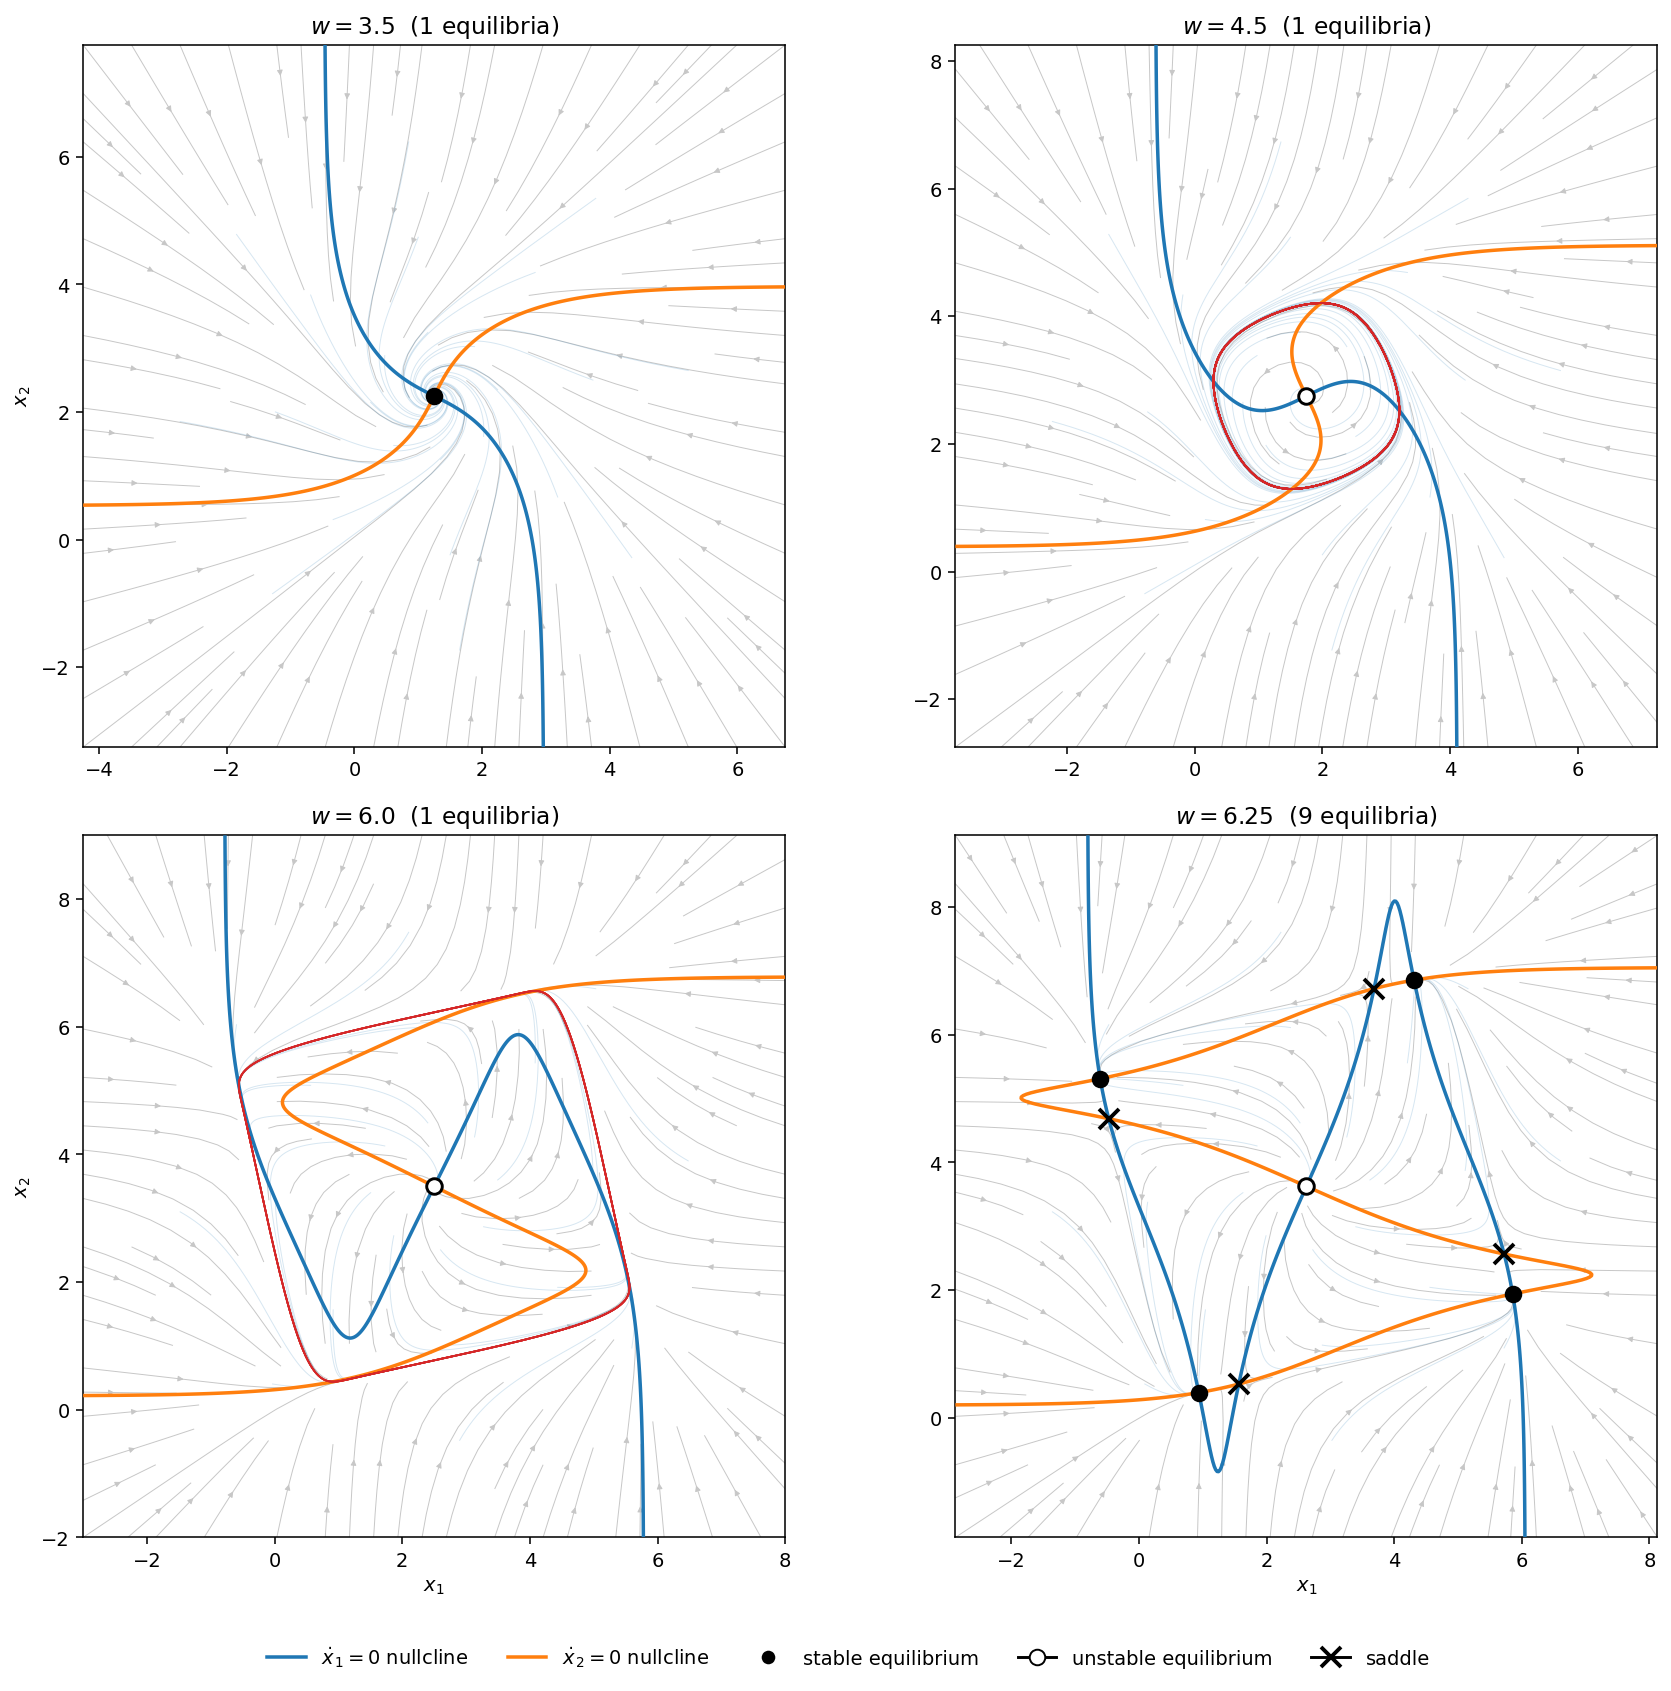
\includegraphics[width=0.8\textwidth]{figures/ctrnn_2x2_panel.png}
  \end{center}
  \caption{A Hopf bifurcation occurs at $w=4$, but the limit cycle is annihilated at $w=6.25$.}
  \label{fig:hopf_bifurcation}
\end{figure*}

While our work in this section has provided an existence proof that CTRNNs can emit periodic dynamics as characterized by stable limit cycles via Hopf bifurcations, the counterexample in Fig.~\ref{fig:hopf_bifurcation} rules out the potential of finding parameter spaces where Hopf bifurcations occur to infer that CTRNNs exhibit periodic dynamics. Hence, in the next section, we develop a Poincar\'e-map-based method for identifying and characterizing periodic dynamics in CTRNNs.

\section{Oscillatory Solutions in Task-Optimized CTRNNs}


% ============================================================
\clearpage
\bibliography{references}
% ============================================================

\end{document}